\documentclass[aspectratio=169, 11pt]{beamer}

% --- Packages & Setup ---
\usepackage[utf8]{inputenc}
\usepackage[T1]{fontenc}
\usepackage{amsmath}
\usepackage{xcolor}
\usepackage{booktabs}
\usepackage{graphicx}
\usepackage{tikz}
\usetikzlibrary{calc,arrows.meta,shapes.geometric}

\graphicspath{{../}{./}}

% Try loading Open Sans; fallback if missing
\IfFileExists{opensans.sty}{\usepackage[default,scale=0.95]{opensans}}{}

% --- Branding Colors ---
\definecolor{amritaMaroon}{HTML}{A4123F}

% --- Diagram Colors (cyan = battgpt-local extension, grey = EMMO / imported) ---
\definecolor{battCyan}{HTML}{DFF6F5}
\definecolor{battCyanLine}{HTML}{2E8B8B}
\definecolor{emmoGrey}{HTML}{EFEFEF}
\definecolor{emmoGreyLine}{HTML}{888888}
\definecolor{flowGrey}{HTML}{555555}

% --- Architecture layer palette ---
\definecolor{condFill}{HTML}{FCEFD5}   \definecolor{condLine}{HTML}{B8891F}
\definecolor{trainFill}{HTML}{EFE6F7}  \definecolor{trainLine}{HTML}{7E5CA6}
\definecolor{genFill}{HTML}{F8E1E8}    \definecolor{genLine}{HTML}{A4123F}
\definecolor{valFill}{HTML}{E3EDF9}    \definecolor{valLine}{HTML}{3F6FA8}

% --- Theme Setup ---
\usetheme{Madrid}
\usecolortheme[named=amritaMaroon]{structure}
\setbeamertemplate{navigation symbols}{}
\setbeamertemplate{footline}[frame number]

% --- Shared diagram node styles ---
\tikzset{
  battbox/.style={rectangle, rounded corners=1.5pt, draw=battCyanLine, fill=battCyan, line width=0.5pt, align=center, font=\tiny, text width=2.0cm, inner sep=2.5pt},
  emmobox/.style={rectangle, rounded corners=1.5pt, draw=emmoGreyLine, fill=emmoGrey, line width=0.5pt, align=center, font=\tiny, text width=2.2cm, inner sep=2.5pt},
  gapbox/.style={rectangle, rounded corners=1.5pt, draw=amritaMaroon, fill=white, line width=0.5pt, dashed, align=center, font=\tiny, text width=2.2cm, inner sep=2.5pt},
  flowarrow/.style={-{Latex[length=1.6mm,width=1.2mm]}, line width=0.5pt, draw=flowGrey},
  % --- architecture diagram styles ---
  archnode/.style 2 args={rectangle, rounded corners=1.5pt, draw=#1, fill=#2, line width=0.5pt, align=center, font=\tiny, text width=2.2cm, minimum height=0.95cm, inner sep=2.5pt},
  archstore/.style 2 args={cylinder, shape border rotate=90, aspect=0.2, draw=#1, fill=#2, line width=0.5pt, align=center, font=\tiny, minimum width=2.5cm, minimum height=0.95cm, inner sep=2pt},
  layerbox/.style={rectangle, draw=#1, dashed, dash pattern=on 2pt off 1.6pt, line width=0.5pt, rounded corners=2pt},
  layerlabel/.style={font=\tiny\bfseries, text=#1, anchor=north west, inner sep=1.5pt},
  archlabel/.style={font=\tiny, text=flowGrey, inner sep=1.5pt},
}
\newcommand{\swatch}[2]{\tikz[baseline=-0.45ex]{\fill[#1] (0,0) rectangle (0.28,0.28); \draw[#2,line width=0.4pt] (0,0) rectangle (0.28,0.28);}}

\begin{document}
% --- CUSTOM TITLE SLIDE (Research) ---
\begin{frame}
    % Corner Box Indicator
    \begin{tikzpicture}[remember picture,overlay]
        \node[fill=amritaMaroon, text=white, font=\bfseries\footnotesize, anchor=north east, rounded corners=2pt, inner sep=5pt]
        at ($(current page.north east) + (-0.2cm,-0.2cm)$)
        {Type 1: Research Project};
    \end{tikzpicture}

    \centering
    
\includegraphics[width=2.8cm]{logo.png}
    \vspace{0.1cm}

    {\large \textbf{\textcolor{amritaMaroon}{Knowledge-Driven Representation and Analysis of Battery Cathode Materials for Accelerated Discovery}}} \\
    \vspace{0.05cm}
    {\footnotesize \textbf{23CSE498 -- Project Phase 2 (Panel Review 1)} \quad | \quad \textbf{Team Number: 25}} \\
    \vspace{0.15cm}

    % Student Table
    \begin{table}
        \centering
        \footnotesize
        \renewcommand{\arraystretch}{1.05}
        \begin{tabular}{|c|c|l|}
            \hline
            \textbf{S.No} & \textbf{Register Number} & \textbf{Student Name} \\
            \hline
            1 & CB.SC.U4CSE23104 & Akshay KS \\
            \hline
            2 & CB.SC.U4CSE23138 & R.D.Tarun \\
            \hline
            3 & CB.SC.U4CSE23142 & S Ajeth \\
            \hline
            4 & CB.SC.U4CSE23145 & Sarvesha NK \\
            \hline
            5 & CB.SC.U4CSE23146 & Shantharam P \\
            \hline
        \end{tabular}
    \end{table}
    \vspace{0.1cm}
    \begin{columns}
\column{0.5\textwidth}
\centering
Guide: \textbf{Dr. Gowtham R} \\
{\footnotesize Associate Professor, Department of CSE}

\column{0.5\textwidth}
\centering
Co-Guide: \textbf{Dr. M. Ulaganathan} \\
{\footnotesize Associate Professor, Department of Physics}
\end{columns}

\vspace{0.2cm}
{\footnotesize September 15, 2026}
\end{frame}

% ============================================================
% SLIDE: INTRODUCTION
% ============================================================

\begin{frame}{Introduction}
\framesubtitle{Knowledge-driven generation of stable battery cathode candidates}
\footnotesize
\begin{itemize}\itemsep0.5em
    \item Discovering viable battery cathode materials by trial and error is slow -- most candidates fail on structural or chemical grounds that domain knowledge could have ruled out early.
    \item \textbf{Our approach:} encode that domain knowledge as an ontology, embed it as a continuous conditioning signal, and use it to steer a pretrained crystal-generation model toward candidates that respect it.
    \item Generated formulas are carried through to real 3D structures and screened down to DFT-validated, experimentally testable candidates.
    \item The rest of this talk walks through each stage: the knowledge layer, the embedding, the conditioning mechanism, and the generation-to-validation pipeline.
\end{itemize}
\end{frame}

% ============================================================
% SLIDE: PROBLEM STATEMENT
% ============================================================

\begin{frame}{Problem Statement}
\framesubtitle{What the knowledge-driven discovery pipeline needs to solve}
\footnotesize
To accelerate discovery of viable battery cathode materials, the pipeline must:
\begin{itemize}\itemsep0.5em
    \item Unify heterogeneous structural, computational, and experimental data into a single, queryable knowledge base.
    \item Turn that knowledge into a continuous signal a generative model can actually condition on, not just a static schema.
    \item Steer crystal generation toward structurally and chemically valid candidates, instead of searching blindly.
    \item Carry generated formulas through to real 3D structures and screen them for stability and synthesizability.
    \item Close the loop with DFT validation and, where possible, experimental confirmation.
\end{itemize}
\end{frame}

\begin{frame}{Application Architecture \& Workflow Design}
\framesubtitle{}
\vfill
\resizebox{0.98\linewidth}{!}{%
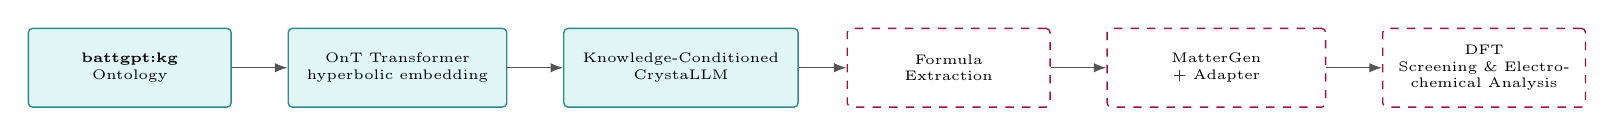
\begin{tikzpicture}[x=1cm,y=1cm]
  \node[battbox, text width=2.4cm, minimum height=1.0cm] (kg) at (0,0) {\textbf{battgpt:kg} \\ Ontology};
  \node[battbox, text width=2.6cm, minimum height=1.0cm] (ont) at (3.4,0) {OnT Transformer \\ {\tiny hyperbolic embedding}};
  \node[battbox, text width=2.8cm, minimum height=1.0cm] (crystallm) at (7.0,0) {Knowledge-Conditioned \\ CrystaLLM};
  \node[gapbox, text width=2.4cm, minimum height=1.0cm] (extract) at (10.4,0) {Formula \\ Extraction};
  \node[gapbox, text width=2.6cm, minimum height=1.0cm] (matter) at (13.8,0) {MatterGen \\ + Adapter};
  \node[gapbox, text width=2.4cm, minimum height=1.0cm] (dft) at (17.2,0) {DFT \\ Screening \& Electrochemical Analysis};

  \foreach \a/\b in {kg/ont, ont/crystallm, crystallm/extract, extract/matter, matter/dft} { \draw[flowarrow] (\a) -- (\b); }
\end{tikzpicture}}
\vfill
{\footnotesize Domain knowledge is embedded and used to condition crystal generation; the resulting formulas are carried through to real 3D structures and screened down to validated candidates -- each stage is detailed in the sections that follow.}
\vfill
{\scriptsize \swatch{battCyan}{battCyanLine} knowledge \& conditioning path \qquad \swatch{white}{amritaMaroon} downstream generation \& validation}
\end{frame}

\section{Implementation Progress}

\begin{frame}{Implementation Progress: Module-Level Status}
    \framesubtitle{Component-by-component state of the knowledge-conditioned pipeline}
    \vspace{-0.1cm}
    \begin{table}
        \centering
        \scriptsize
        \renewcommand{\arraystretch}{1.15}
        \begin{tabular}{p{3.4cm} p{7.2cm} c}
            \toprule
            \textbf{Module / Component} & \textbf{Current Implementation State} & \textbf{Status} \\
            \midrule
            Ontology (\texttt{battgpt:kg}) & v0.3.2 -- 894 triples, 32 classes, 28 object / 30 datatype properties; two local extensions; cathode instances populated & Functional \\
            OnT hyperbolic embedding & Poincar\'e ball embeddings over the merged ontology closure; centripetal radial ordering verified & Functional \\
            Ontology $\to$ pipeline bridge & Deterministic ancestor traversal, memory-bank construction, persisted run manifest & Functional \\
            Conditioning layer & Zero-initialised gated cross-attention wired into frozen CrystaLLM blocks & Integrated \\
            Structure-family classifier & pymatgen space-group + composition rules across all nine leaf families & Functional \\
            Generation \& validation & End-to-end CIF generation with an independently grounded validation gate & In Progress \\
            MatterGen handoff & Formula extraction to seed the team's MatterGen track & Planned \\
            \bottomrule
        \end{tabular}
    \end{table}

\end{frame}

\begin{frame}{What is EMMO?}
\framesubtitle{Scope, current extensions, and the case for extending it further}
\begin{columns}[T]
    \column{0.48\textwidth}
    \footnotesize
    \begin{itemize}\itemsep0.3em
        \item \textbf{EMMO}~\cite{emmo2024}: a foundational, axiomatic upper ontology for materials science, grounded in physics and analytical philosophy.
        \item \textbf{Mature domains reused as-is:} domain-battery (BattINFO-aligned~\cite{clark2022battinfo}), domain-electrochemistry, domain-chemical-substance.
        \item \textbf{domain-crystallography is not usable:} an explicit work-in-progress v0.1.0 draft -- confirmed by direct inspection, not imported by anyone.
        \item \textbf{Why we extend:} generation needs machine-readable crystallographic structure aligned with DFT output, and a structure-family classification vocabulary -- neither exists upstream.
       \item Battery chemistry is \emph{already} covered.
    \end{itemize}

    \column{0.5\textwidth}
    \centering
    \resizebox{\linewidth}{!}{%
    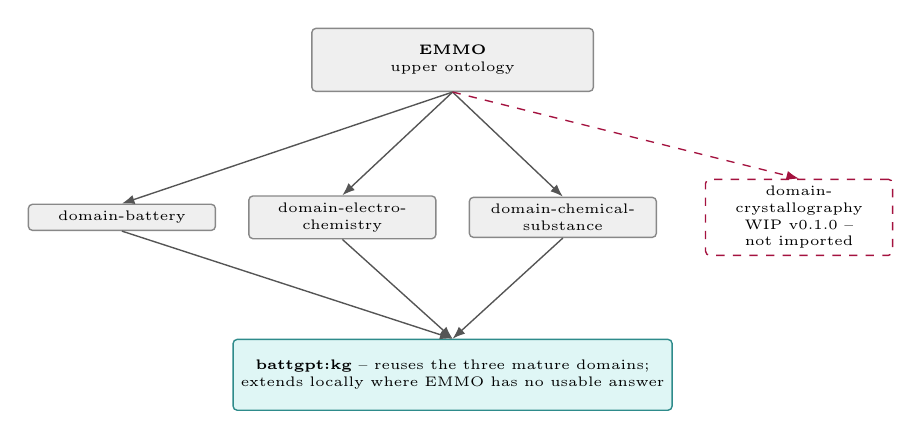
\begin{tikzpicture}[x=1cm,y=1cm]
      \node[emmobox, text width=3.4cm, minimum height=0.8cm] (emmo) at (0,4.2) {\textbf{EMMO} \\ upper ontology};

      \node[emmobox] (bat) at (-4.2,2.2) {domain-battery};
      \node[emmobox] (echem) at (-1.4,2.2) {domain-electro-chemistry};
      \node[emmobox] (chsub) at (1.4,2.2) {domain-chemical-substance};
      \node[gapbox] (cryst) at (4.4,2.2) {domain-crystallography \\ {\tiny WIP v0.1.0 -- not imported}};

      \draw[flowarrow] (emmo.south) -- (bat.north);
      \draw[flowarrow] (emmo.south) -- (echem.north);
      \draw[flowarrow] (emmo.south) -- (chsub.north);
      \draw[flowarrow, dashed, draw=amritaMaroon] (emmo.south) -- (cryst.north);

      \node[battbox, text width=5.4cm, minimum height=0.9cm] (kg) at (0,0.2) {\textbf{battgpt:kg} -- reuses the three mature domains; extends locally where EMMO has no usable answer};

      \draw[flowarrow] (bat.south) -- (kg.north);
      \draw[flowarrow] (echem.south) -- (kg.north);
      \draw[flowarrow] (chsub.south) -- (kg.north);
    \end{tikzpicture}}
    \\[3pt]
    {\tiny \swatch{emmoGrey}{emmoGreyLine} EMMO / mature, reused \quad \swatch{white}{amritaMaroon} WIP, not usable \quad \swatch{battCyan}{battCyanLine} battgpt-local}
\end{columns}
\end{frame}

% ============================================================
% SLIDE: COMPETENCY QUESTIONS
% ============================================================
\begin{frame}{Competency Questions}
\framesubtitle{What the ontology must be able to answer}
\footnotesize
\textbf{Crystallographic structure}
\begin{itemize}\itemsep0.15em
    \item CQ1. What are the unit cell parameters and space group of a given crystal structure?
    \item CQ2. Which sites and species occupy the structure, at what fractional coordinates, and in what coordination geometry?
    \item CQ3. Which bonds exist between which sites, at what distance, and by what determination method?
    \item CQ4. What DFT-calculated properties (band gap, formation energy, energy above hull, bulk/shear modulus) does a material have, under which computational method?
\end{itemize}
\vspace{0.2cm}
\textbf{Structural classification}
\begin{itemize}\itemsep0.15em
    \item CQ5. Which structural-prototype family (layered oxide, olivine, spinel, garnet, NASICON, sulfide superionic, \dots) does a structure belong to?
    \item CQ6. Is a material's family classification unique and reasoner-checkable, not just convention?
\end{itemize}
\vspace{0.2cm}
\textbf{Battery chemistry (reused, not extended)}
\begin{itemize}\itemsep0.15em
    \item CQ7. What functional role (positive electrode, negative electrode, electrolyte, separator) does a material play in a cell?
    \item CQ8. What are a cell's rated electrochemical properties (capacity, voltage, ionic conductivity, \dots)?
\end{itemize}
\end{frame}

% ============================================================
% SLIDE: SCHEMA OVERVIEW -- TWO EXTENSIONS
% ============================================================
\begin{frame}{Ontology Schema Overview}
\framesubtitle{Two local extensions, one domain reused as-is}
\centering
\resizebox{0.85\linewidth}{!}{%
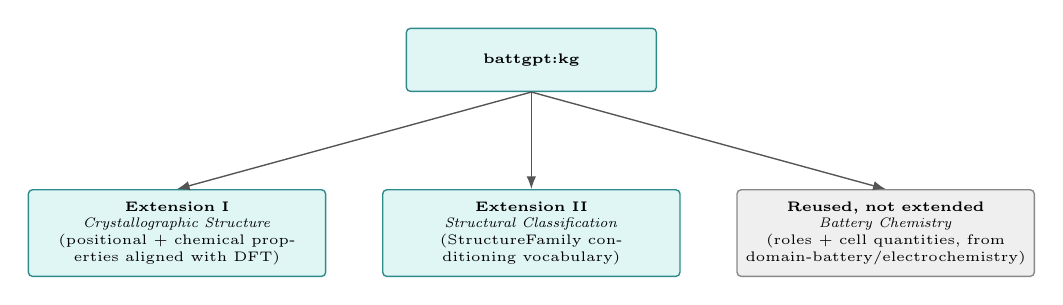
\begin{tikzpicture}[x=1cm,y=1cm]
  \node[battbox, text width=3.0cm, minimum height=0.8cm] (kg) at (0,3.4) {\textbf{battgpt:kg}};

  \node[battbox, text width=3.6cm, minimum height=1.1cm] (cryst) at (-4.5,1.2) {\textbf{Extension I} \\ \textit{Crystallographic Structure} \\ {\tiny (positional + chemical properties aligned with DFT)}};
  \node[battbox, text width=3.6cm, minimum height=1.1cm] (struct) at (0,1.2) {\textbf{Extension II} \\ \textit{Structural Classification} \\ {\tiny (StructureFamily conditioning vocabulary)}};
  \node[emmobox, text width=3.6cm, minimum height=1.1cm] (chem) at (4.5,1.2) {\textbf{Reused, not extended} \\ \textit{Battery Chemistry} \\ {\tiny (roles + cell quantities, from domain-battery/electrochemistry)}};

  \draw[flowarrow] (kg.south) -- (cryst.north);
  \draw[flowarrow] (kg.south) -- (struct.north);
  \draw[flowarrow] (kg.south) -- (chem.north);
\end{tikzpicture}}

\vspace{0.4cm}
{\footnotesize \swatch{battCyan}{battCyanLine} defined locally by this project \qquad \swatch{emmoGrey}{emmoGreyLine} imported from EMMO, used as-is}
\end{frame}

% ============================================================
% SLIDE: EXTENSION I -- CRYSTALLOGRAPHIC STRUCTURE
% ============================================================
\begin{frame}{Extension I: Crystallographic Structure}
\framesubtitle{Positional \& chemical properties aligned with DFT-calculated properties}
\centering
\resizebox{0.82\linewidth}{!}{%
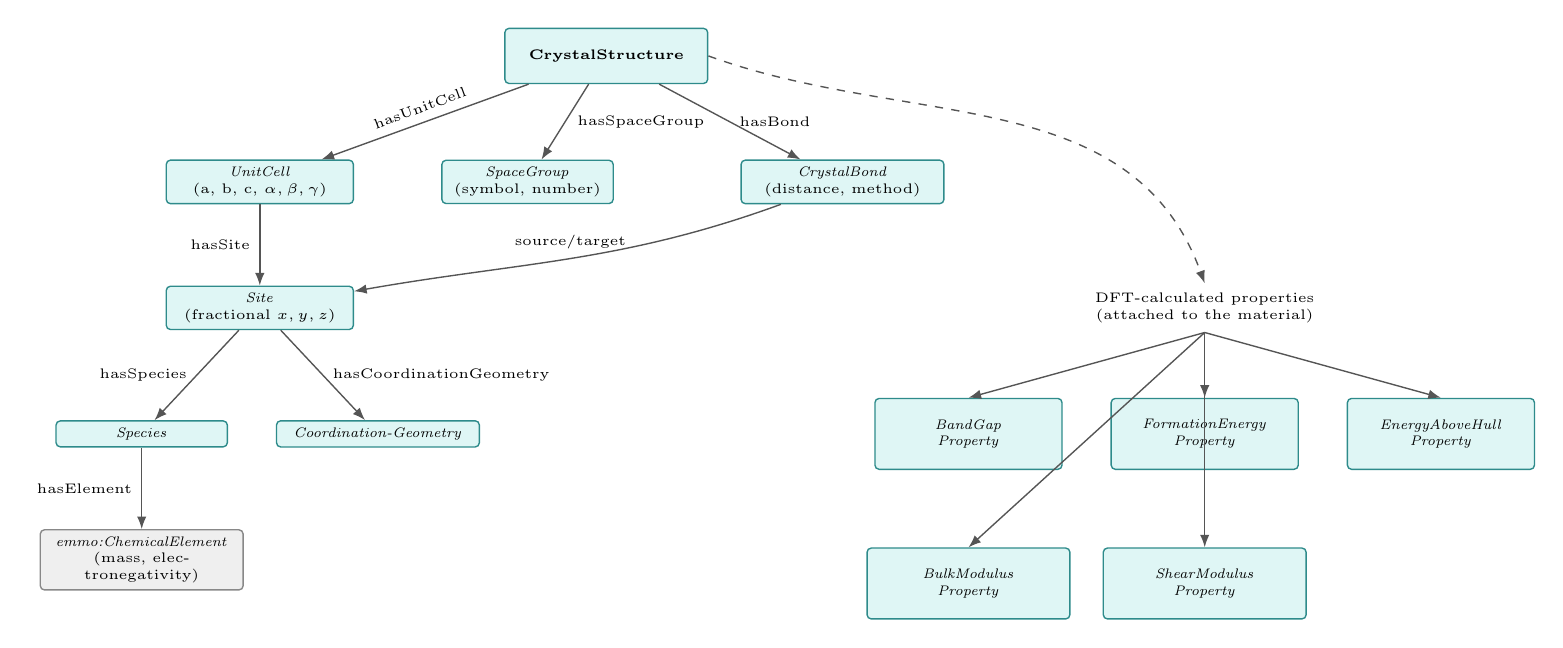
\begin{tikzpicture}[x=1cm,y=1cm]
  \node[battbox, text width=2.4cm, minimum height=0.7cm] (cs) at (0,5.4) {\textbf{CrystalStructure}};

  \node[battbox, text width=2.2cm] (uc) at (-4.4,3.8) {\textit{UnitCell} \\ {\tiny (a, b, c, $\alpha,\beta,\gamma$)}};
  \node[battbox, text width=2.0cm] (sg) at (-1.0,3.8) {\textit{SpaceGroup} \\ {\tiny (symbol, number)}};
  \node[battbox, text width=2.4cm] (cb) at (3.0,3.8) {\textit{CrystalBond} \\ {\tiny (distance, method)}};

  \node[battbox, text width=2.2cm] (site) at (-4.4,2.2) {\textit{Site} \\ {\tiny (fractional $x,y,z$)}};

  \node[battbox, text width=2.0cm] (species) at (-5.9,0.6) {\textit{Species}};
  \node[battbox, text width=2.4cm] (cg) at (-2.9,0.6) {\textit{Coordination-Geometry}};
  \node[emmobox, text width=2.4cm] (elem) at (-5.9,-1.0) {\textit{emmo:ChemicalElement} \\ {\tiny (mass, electronegativity)}};

  \draw[flowarrow] (cs) -- node[above,sloped,font=\tiny]{hasUnitCell} (uc);
  \draw[flowarrow] (cs) -- node[right,font=\tiny,xshift=1pt]{hasSpaceGroup} (sg);
  \draw[flowarrow] (cs) -- node[right,font=\tiny]{hasBond} (cb);
  \draw[flowarrow] (uc) -- node[left,font=\tiny]{hasSite} (site);
  \draw[flowarrow] (cb) to[out=200,in=10] node[above,font=\tiny]{source/target} (site);
  \draw[flowarrow] (site) -- node[left,font=\tiny]{hasSpecies} (species);
  \draw[flowarrow] (site) -- node[right,font=\tiny]{hasCoordinationGeometry} (cg);
  \draw[flowarrow] (species) -- node[left,font=\tiny]{hasElement} (elem);

  \node[battbox, text width=2.2cm, minimum height=0.9cm] (bg) at (4.6,0.6) {\textit{BandGap} \\ \textit{Property}};
  \node[battbox, text width=2.2cm, minimum height=0.9cm] (fe) at (7.6,0.6) {\textit{FormationEnergy} \\ \textit{Property}};
  \node[battbox, text width=2.2cm, minimum height=0.9cm] (eh) at (10.6,0.6) {\textit{EnergyAboveHull} \\ \textit{Property}};
  \node[battbox, text width=2.4cm, minimum height=0.9cm] (bm) at (4.6,-1.3) {\textit{BulkModulus} \\ \textit{Property}};
  \node[battbox, text width=2.4cm, minimum height=0.9cm] (sm) at (7.6,-1.3) {\textit{ShearModulus} \\ \textit{Property}};

  \node[align=center,font=\tiny] (dft) at (7.6,2.2) {DFT-calculated properties \\ (attached to the material)};
  \draw[flowarrow, dashed] (cs.east) to[out=-20,in=110] (dft.north);
  \foreach \c in {bg,fe,eh,bm,sm} { \draw[flowarrow] (dft.south) -- (\c.north); }
\end{tikzpicture}}

\vspace{0.05cm}
{\scriptsize \textbf{Justification:} We ground \texttt{CrystalStructure} directly under \texttt{owl:Thing} because EMMO's domain-crystallography is still an unreleased v0.1.0 draft that nothing else imports. This is the only place we represent positional and chemical structure in a form that lines up with what DFT actually computes.}
\end{frame}

% ============================================================
% SLIDE: EXTENSION II -- STRUCTURAL CLASSIFICATION
% ============================================================
\begin{frame}{Extension II: Structural Classification}
\framesubtitle{The StructureFamily conditioning vocabulary}
\centering
\resizebox{0.97\linewidth}{!}{%
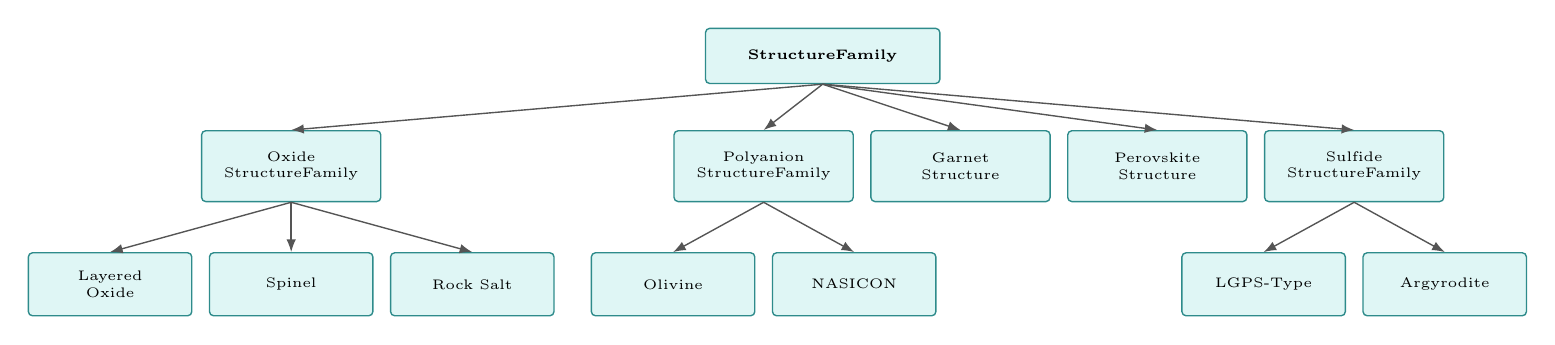
\begin{tikzpicture}[x=1cm,y=1cm]
  \node[battbox, text width=2.8cm, minimum height=0.7cm] (root) at (0,4.0) {\textbf{StructureFamily}};

  \node[battbox, text width=2.1cm, minimum height=0.9cm] (oxide) at (-6.75,2.6) {Oxide\\StructureFamily};
  \node[battbox, text width=2.1cm, minimum height=0.9cm] (poly)  at (-0.75,2.6) {Polyanion\\StructureFamily};
  \node[battbox, text width=2.1cm, minimum height=0.9cm] (garnet) at (1.75,2.6) {Garnet\\Structure};
  \node[battbox, text width=2.1cm, minimum height=0.9cm] (perov)  at (4.25,2.6) {Perovskite\\Structure};
  \node[battbox, text width=2.1cm, minimum height=0.9cm] (sulf)   at (6.75,2.6) {Sulfide\\StructureFamily};

  \node[battbox, text width=1.9cm, minimum height=0.8cm] (layered) at (-9.05,1.1) {Layered\\Oxide};
  \node[battbox, text width=1.9cm, minimum height=0.8cm] (spinel)  at (-6.75,1.1) {Spinel};
  \node[battbox, text width=1.9cm, minimum height=0.8cm] (rocksalt)  at (-4.45,1.1) {Rock Salt};
  \node[battbox, text width=1.9cm, minimum height=0.8cm] (olivine) at (-1.9,1.1) {Olivine};
  \node[battbox, text width=1.9cm, minimum height=0.8cm] (nasicon) at (0.4,1.1) {NASICON};
  \node[battbox, text width=1.9cm, minimum height=0.8cm] (lgps) at (5.6,1.1) {LGPS-Type};
  \node[battbox, text width=1.9cm, minimum height=0.8cm] (argy) at (7.9,1.1) {Argyrodite};

  \foreach \c in {oxide,poly,garnet,perov,sulf} { \draw[flowarrow] (root.south) -- (\c.north); }
  \foreach \c in {layered,spinel,rocksalt} { \draw[flowarrow] (oxide.south) -- (\c.north); }
  \foreach \c in {olivine,nasicon} { \draw[flowarrow] (poly.south) -- (\c.north); }
  \foreach \c in {lgps,argy} { \draw[flowarrow] (sulf.south) -- (\c.north); }
\end{tikzpicture}}

\vspace{0.15cm}
{\scriptsize Each leaf is anchored to a canonical example from our pipeline's curated Materials Project records~\cite{jain2013materialsproject} -- LiCoO$_2$/LiNiO$_2$, LiMn$_2$O$_4$/Li$_4$Ti$_5$O$_{12}$, LiFePO$_4$/NaFePO$_4$, Na$_3$V$_2$(PO$_4$)$_3$, LGPS, LLZO. All nine leaves are \texttt{owl:AllDisjointClasses}}

\vspace{0.1cm}
{\scriptsize \textbf{Justification:} We checked every relevant EMMO domain -- the ones we import (chemical-substance, battery, electrochemistry) and the not-yet-usable domain-crystallography draft -- and none of them define this structural-prototype vocabulary, so we built it locally. This is the conditioning vocabulary CrystaLLM and OnT need; deliberately the deepest subclass hierarchy in the ontology.}
\end{frame}

% ============================================================
% SLIDE: SCOPE & LIMITATIONS
% ============================================================
\begin{frame}{Scope \& Limitations}
\framesubtitle{Where the schema currently stands}
\footnotesize
\begin{itemize}\itemsep0.5em
    \item \textbf{Instances are populated, but only a cathode slice:} real materials (e.g.\ LiFePO$_4$) are populated end-to-end, not yet spanning every StructureFamily leaf or the electrolyte/separator roles.
    \item \textbf{Few places still need formal constraints:} e.g.\ DFT properties already carry a value and a unit in practice, but the ontology doesn't yet require it -- this is one of several such gaps, and tightening them is an ongoing refinement.
    \item \textbf{Provenance is tracked, reconciliation is not:} each property and bond records its source method, but comparing the same quantity across multiple databases for one material is still open.
    \item \textbf{Consistency is now reasoner-checked:} every ontology change is validated with ELK~\cite{kazakov2014elk} (EL profile) and HermiT (full consistency) before it's applied -- zero new unsatisfiable classes introduced so far.
\end{itemize}
\end{frame}

% ============================================================
% SLIDE: ONT HYPERBOLIC EMBEDDINGS
% ============================================================
\section{CrystaLLM}


% ============================================================
% SLIDE: THE NEED FOR ONTOLOGY EMBEDDING
% ============================================================
\begin{frame}{The Core Question: How Does a Model Understand an Ontology?}
\framesubtitle{Moving from human-readable symbolic graphs to machine-executable representations}

\vspace{-0.2cm}
\begin{columns}[T]
    \column{0.49\textwidth}
    \scriptsize
    \textbf{1. It Must Understand English Semantics}
    \begin{itemize}\itemsep0.15em
        \item Classes carry rich descriptive domain text (\textit{``delithiated high-nickel layered oxide''}).
        \item Relations encode physical logic (\textit{hasCoordinationGeometry}) requiring textual grounding.
        \item \textbf{Failure of pure IDs:} Discrete graph tokens discard chemical and linguistic meanings.
    \end{itemize}

    \column{0.49\textwidth}
    \scriptsize
    \textbf{2. It Must Preserve Strict Hierarchies}
    \begin{itemize}\itemsep0.15em
        \item Subsumption is asymmetric: every \textit{Layered Oxide} is an \textit{Oxide}, but not vice-versa.
        \item Distance must reflect taxonomic depth and shared parentage rather than surface word similarity.
        \item \textbf{Failure of standard PLMs:} Flat Euclidean space causes metric distortion and tree crowding.
    \end{itemize}
\end{columns}

\vspace{0.15cm}
\begin{beamercolorbox}[rounded=true, sep=2.5pt]{block body}
    \centering\scriptsize
    \textbf{The Challenge:} How do we map symbolic logic into a continuous space that preserves \textbf{both natural-language semantics} and \textbf{hierarchical tree geometry}?
\end{beamercolorbox}

\vspace{0.15cm}
\centering
\resizebox{0.92\linewidth}{!}{%
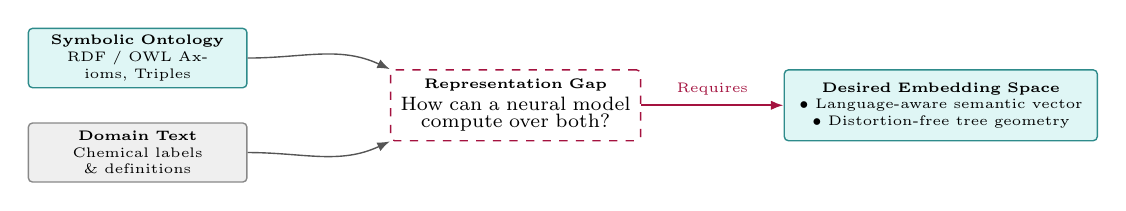
\begin{tikzpicture}[x=1cm,y=1cm]
  % Inputs
  \node[battbox, text width=2.6cm, minimum height=0.75cm] (ont) at (0, 0.6) {\textbf{Symbolic Ontology} \\ {\tiny RDF / OWL Axioms, Triples}};
  \node[emmobox, text width=2.6cm, minimum height=0.75cm] (txt) at (0, -0.6) {\textbf{Domain Text} \\ {\tiny Chemical labels \& definitions}};

  % Center Problem Box
  \node[gapbox, text width=3.0cm, minimum height=0.9cm] (quest) at (4.8, 0) {\textbf{Representation Gap} \\ {\scriptsize How can a neural model \\ compute over both?}};

  % Target Requirements
  \node[battbox, text width=3.8cm, minimum height=0.9cm] (target) at (10.2, 0) {\textbf{Desired Embedding Space} \\ {\tiny $\bullet$ Language-aware semantic vector \\ $\bullet$ Distortion-free tree geometry}};

  % Arrows
  \draw[flowarrow] (ont.east) to[out=0, in=155] (quest.north west);
  \draw[flowarrow] (txt.east) to[out=0, in=-155] (quest.south west);
  \draw[flowarrow, draw=amritaMaroon, line width=0.8pt] (quest) -- node[above, font=\tiny, text=amritaMaroon]{Requires} (target);
\end{tikzpicture}}
\end{frame}

\begin{frame}{OnT: Hyperbolic Ontology Embeddings}
\framesubtitle{Unifying language models and axiomatic hierarchies in non-Euclidean space}

\vspace{-0.35cm}
\begin{columns}[T]
    \column{0.52\textwidth}
    \scriptsize
    \textbf{What is OnT?}
    \begin{itemize}\itemsep0.05em
        \item Tunes a \textbf{PLM} via geometric modeling in hyperbolic space.
        \item Preserves Description Logic $\mathcal{EL}$ axioms ($C \sqsubseteq D$, $\exists r.C$, $C \sqcap D$) and text.
    \end{itemize}

    \vspace{0.08cm}
    \textbf{How It Works}
    \begin{itemize}\itemsep0.05em
        \item \textbf{Verbalizer + PLM:} Converts complex concepts into text ($\mathcal{V}(C)$).
        \item \textbf{Roles as Rotations:} Models roles via rotation $R(\Theta_r)$ and scale $k_r$.
        \item \textbf{Hierarchy Losses:} Optimizes via \textit{Contrastive} and \textit{Centripetal} losses.
    \end{itemize}

    \vspace{0.08cm}
    \textbf{Why Hyperbolic Space?}
    \begin{itemize}\itemsep0.05em
        \item \textbf{Exponential Volume:} Radius growth matches tree branching rates.
        \item \textbf{Zero Leaf Crowding:} Prevents metric collapse between deep leaves.
    \end{itemize}

    \column{0.46\textwidth}
    \centering
    \vspace{0.15cm}
    \resizebox{0.78\linewidth}{!}{%
    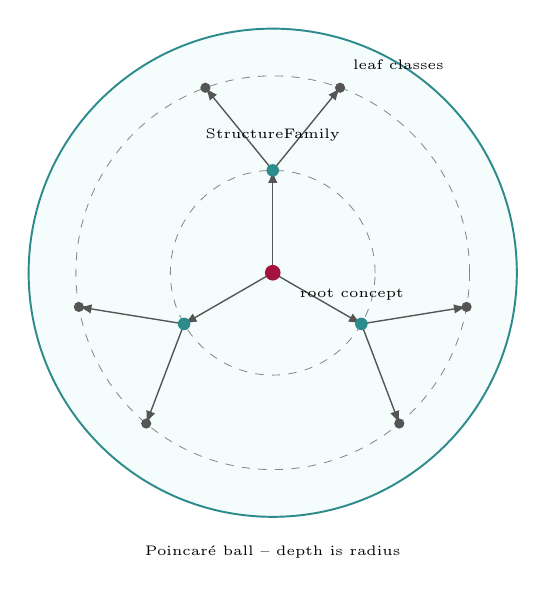
\begin{tikzpicture}[x=1cm,y=1cm]
      \fill[battCyan, opacity=0.35] (0,0) circle (3.1);
      \draw[battCyanLine, line width=0.7pt] (0,0) circle (3.1);
      \draw[emmoGreyLine, dashed, line width=0.3pt] (0,0) circle (1.3);
      \draw[emmoGreyLine, dashed, line width=0.3pt] (0,0) circle (2.5);

      \foreach \a in {90,210,330} { \draw[flowarrow] (0,0) -- (\a:1.3); }
      \draw[flowarrow] (90:1.3) -- (70:2.5);
      \draw[flowarrow] (90:1.3) -- (110:2.5);
      \draw[flowarrow] (210:1.3) -- (190:2.5);
      \draw[flowarrow] (210:1.3) -- (230:2.5);
      \draw[flowarrow] (330:1.3) -- (310:2.5);
      \draw[flowarrow] (330:1.3) -- (350:2.5);

      \node[circle, fill=amritaMaroon, inner sep=2.0pt] at (0,0) {};
      \foreach \a in {90,210,330} { \node[circle, fill=battCyanLine, inner sep=1.6pt] at (\a:1.3) {}; }
      \foreach \a in {70,110,190,230,310,350} { \node[circle, fill=flowGrey, inner sep=1.3pt] at (\a:2.5) {}; }

      \node[font=\tiny, anchor=west] at (0.22,-0.28) {root concept};
      \node[font=\tiny, anchor=south] at (90:1.55) {StructureFamily};
      \node[font=\tiny, anchor=south west] at (70:2.62) {leaf classes};
      \node[font=\tiny, anchor=north] at (0,-3.35) {Poincar\'e ball -- depth is radius};
    \end{tikzpicture}}
\end{columns}
\end{frame}

% ============================================================
% SLIDE: WHY KG IN PARALLEL
% ============================================================
\begin{frame}{Why a Knowledge Graph, Not Only the Ontology}
\framesubtitle{Same pipeline, two objects: schema vs instances}
\begin{columns}[T]
    \column{0.52\textwidth}
    \footnotesize
    \textbf{The missing instance information}
    \begin{itemize}\itemsep0.22em
        \item \textbf{OnT encodes the TBox:} concepts, hierarchy, and ontology relations~\cite{yang2025ont}.
        \item A \textbf{class embedding is shared:} LiFePO$_4$ and NMC811 may both be instances of \texttt{Substance}, but their properties differ.
        \item The populated KG provides the \textbf{ABox:} materials, crystals, properties, and relations.
    \end{itemize}
    \vspace{0.2cm}
    \textbf{Parallel, not a replacement}
    \begin{itemize}\itemsep0.22em
        \item \textbf{TBox / Ontology:} what kinds of things exist and how they are related.
        \item \textbf{ABox / KG:} which specific things exist and what is true about them.
        \item Encode both and provide the \textbf{material-specific representations} to the cross-attention injector in CrystaLLM~\cite{antunes2024crystallm}.
    \end{itemize}

    \column{0.46\textwidth}
    \centering
    \vspace{0.25cm}
    \resizebox{0.92\linewidth}{!}{%
    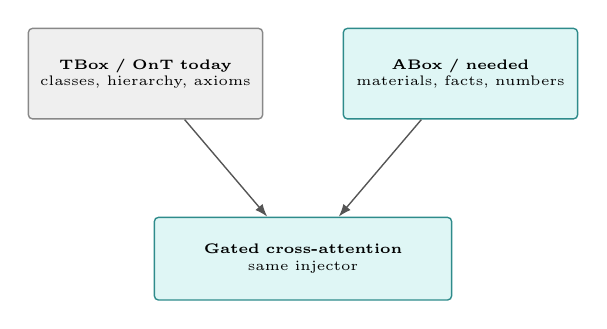
\begin{tikzpicture}[x=1cm,y=1cm]
      \node[emmobox, text width=2.8cm, minimum height=1.15cm] (tbox) at (-2.0,2.0) {\textbf{TBox / OnT today} \\ {\tiny classes, hierarchy, axioms}};
      \node[battbox, text width=2.8cm, minimum height=1.15cm] (abox) at (2.0,2.0) {\textbf{ABox / needed} \\ {\tiny materials, facts, numbers}};
      \node[battbox, text width=3.6cm, minimum height=1.05cm] (ca) at (0,-0.35) {\textbf{Gated cross-attention} \\ {\tiny same injector}};
      \draw[flowarrow] (tbox) -- (ca);
      \draw[flowarrow] (abox) -- (ca);
    \end{tikzpicture}}
    \\[4pt]
    {\tiny \swatch{emmoGrey}{emmoGreyLine} schema already encoded \quad \swatch{battCyan}{battCyanLine} instance track}
\end{columns}
\end{frame}

% ============================================================
% SLIDE: EXISTING ENCODERS
% ============================================================
\begin{frame}{Existing Encoders: Strengths and Gaps}
\framesubtitle{No single method combines all signals required by our KG}

\vspace{-0.05cm}

\begin{table}
    \centering
    \scriptsize
    \renewcommand{\arraystretch}{1.18}
    \begin{tabular}{p{2.7cm} p{5.7cm} p{5.2cm}}
        \toprule
        \textbf{Method} & \textbf{What it captures} & \textbf{Gap for our setting} \\
        \midrule

        \textbf{BoxEL}~\cite{xiong2022boxel} &
        Classes as boxes, individuals as points, and
        relations as transformations.
        \textbf{TBox + ABox} logical constraints. &
        No native scientific text or dedicated
        numerical representation. \\

        \textbf{Box$^2$EL}~\cite{jackermeier2024dual} &
        Improved EL++ representation with concept boxes,
        individual points, and richer role representation.
        \textbf{TBox + ABox}. &
        No language-model or dedicated
        concrete-value encoder. \\

        \textbf{SimKGC}~\cite{wang2022simkgc} &
        Language-model representations of entity/relation
        text for KG link prediction. &
        No ontology-specific semantics or
        dedicated numerical representation. \\

        \textbf{KEPLER}~\cite{wang2021kepler} &
        Language-model entity descriptions jointly trained
        with TransE for KG representation. &
        Not designed for ontology-specific semantics
        or scientific numerical features. \\

        \textbf{RotatE}~\cite{sun2019rotate} &
        Learned entity/relation embeddings for
        KG structure and link prediction. &
        Does not directly exploit our node types
        or numerical features. \\

        \bottomrule
    \end{tabular}
\end{table}

\vspace{0.15cm}

\begin{center}
{\small
\textbf{Our requirement:}\quad
TBox semantics + ABox instances + scientific attributes
$\rightarrow$ \textbf{material embeddings} for CrystaLLM~\cite{antunes2024crystallm}
(OnT~\cite{yang2025ont} is the encoder we extend)}
\end{center}

\end{frame}


% ============================================================
% SLIDE: PLANNED ONT+ABOX ARCHITECTURE
% ============================================================
\begin{frame}{Planned Architecture: Extending OnT to the Populated KG}
\framesubtitle{Verbalize instances, reuse OnT, add a numerical feature channel}
\begin{columns}[T]
    \column{0.52\textwidth}
    \centering
    \resizebox{0.90\linewidth}{!}{%
    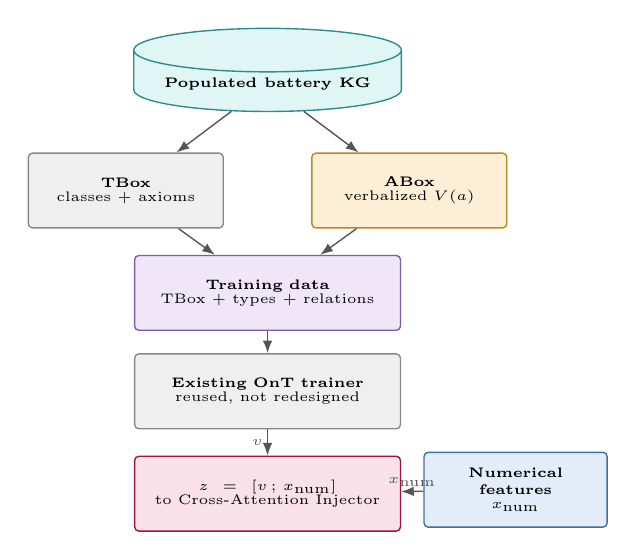
\begin{tikzpicture}[x=1cm,y=1cm]
      \node[archstore={battCyanLine}{battCyan}, minimum width=3.4cm]
      (ttl) at (1.8,5.2)
      {\textbf{Populated battery KG}};

      \node[archnode={emmoGreyLine}{emmoGrey}, text width=2.3cm]
      (tbox) at (0.0,3.85)
      {\textbf{TBox}\\[-1pt] {\tiny classes + axioms}};

      \node[archnode={condLine}{condFill}, text width=2.3cm]
      (abox) at (3.6,3.85)
      {\textbf{ABox}\\[-1pt] {\tiny verbalized $V(a)$}};

      \node[archnode={trainLine}{trainFill}, text width=3.2cm]
      (train) at (1.8,2.55)
      {\textbf{Training data}\\[-1pt] {\tiny TBox + types + relations}};

      \node[archnode={emmoGreyLine}{emmoGrey}, text width=3.2cm]
      (ont) at (1.8,1.3)
      {\textbf{Existing OnT trainer}\\[-1pt] {\tiny reused, not redesigned}};

      \node[archnode={valLine}{valFill}, text width=2.15cm]
      (num) at (4.95,0.05)
      {\textbf{Numerical features}\\[-1pt] {\tiny $x_{\mathrm{num}}$}};

      \node[archnode={genLine}{genFill}, text width=3.2cm]
      (z) at (1.8,0.0)
      {$z=[v\,;\,x_{\mathrm{num}}]$\\[-1pt] {\tiny to Cross-Attention Injector}};

      \draw[flowarrow] (ttl) -- (tbox);
      \draw[flowarrow] (ttl) -- (abox);
      \draw[flowarrow] (tbox) -- (train);
      \draw[flowarrow] (abox) -- (train);
      \draw[flowarrow] (train) -- (ont);
      \draw[flowarrow] (ont) -- node[archlabel,left]{$v$} (z);
      \draw[flowarrow] (num) -- node[archlabel,above]{$x_{\mathrm{num}}$} (z);
    \end{tikzpicture}}

    \column{0.46\textwidth}
    \footnotesize
    \textbf{What we do}
    \begin{itemize}\itemsep0.35em
        \item Keep OnT for the \textbf{TBox}. Verbalize each material and encode it with the \textbf{same PLM/OnT pipeline} -- one encoder, not a second model.
        \item Extend OnT's hierarchy and role losses to ABox types and relations, and evaluate the resulting instance geometry.
        \item After OnT, attach scaled numbers: $v$ is the hyperbolic embedding; $z=[v;x_{\mathrm{num}}]$ is what CrystaLLM sees.
        \item Retrieve \textbf{material-specific} $z$ into the existing Cross-Attention Injector. CrystaLLM stays frozen.
    \end{itemize}
\end{columns}
\end{frame}

\begin{frame}{The Need for a Generative Model?}
\framesubtitle{The gap between a formula and a usable 3D crystal structure}
\footnotesize
\begin{columns}[T]
    \column{0.49\textwidth}
    \textbf{The Problem}
    \begin{itemize}\itemsep0.3em
        \item Our ontology-conditioned pipeline outputs a \textbf{chemical formula} -- not a 3D structure.
        \item Existing databases (Materials Project, ICSD) cover known materials only -- novel cathode candidates are by definition absent.
        \item Brute-force DFT enumeration of all possible structures for a formula is computationally infeasible.
    \end{itemize}

    \column{0.49\textwidth}
    \textbf{What the Model Must Do}
    \begin{itemize}\itemsep0.3em
        \item Given a formula (and optionally a target symmetry), \textbf{propose valid 3D crystal structures} on demand.
        \item Respect crystallographic constraints: space group, Wyckoff sites, unit cell geometry.
        \item Accept external conditioning signals -- our ontology knowledge must actually influence what gets generated.
    \end{itemize}
\end{columns}

\vspace{0.3cm}
\begin{beamercolorbox}[rounded=true, sep=2.5pt]{block body}
    \centering\scriptsize
    \textbf{The question then becomes:} what \emph{type} of generative model satisfies all three requirements?
\end{beamercolorbox}
\end{frame}

% ============================================================
% SLIDE: WHY CRYSTALLM? (Motivating question)
% ============================================================
\begin{frame}{The Core Question: Auto-Regressive Generative Model}
\framesubtitle{From disordered diffusion to exact, conditioned structure generation}

\vspace{-0.2cm}
\begin{columns}[T]
    \column{0.49\textwidth}
    \scriptsize
    \textbf{1. Crystal Generation Must Preserve Symmetry}
    \begin{itemize}\itemsep0.15em
        \item A valid crystal is governed by a space group -- every atomic position is constrained to Wyckoff sites.
        \item Continuous diffusion drifts across 1{,}000 denoising steps, routinely collapsing into disordered $P1$.
        \item \textbf{CrystaLLM emits the space group first:} all coordinates are conditioned on it -- symmetry by construction.
    \end{itemize}

    \column{0.49\textwidth}
    \scriptsize
    \textbf{2. Generation Must Accept External Signals}
    \begin{itemize}\itemsep0.15em
        \item Battery discovery requires steering toward target compositions and structural families -- not random sampling.
        \item Score-function conditioning in diffusion models is incompatible with discrete ontology signals.
        \item \textbf{CrystaLLM accepts a prefix:} formula, space group, or atomic properties -- exactly what our ontology provides.
    \end{itemize}
\end{columns}

\vspace{0.15cm}
\begin{beamercolorbox}[rounded=true, sep=2.5pt]{block body}
    \centering\scriptsize
    \textbf{Key Insight:} CIF text sequences enforce symmetry exactly and accept ontology prefixes naturally -- the right fit for knowledge-conditioned discovery.
\end{beamercolorbox}

\vspace{0.15cm}
\centering
\resizebox{0.88\linewidth}{!}{%
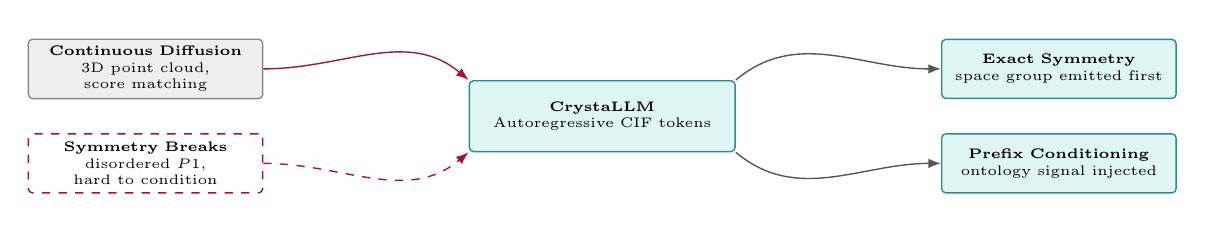
\begin{tikzpicture}[x=1cm,y=1cm]
  \node[emmobox, text width=2.8cm, minimum height=0.75cm] (diff) at (0, 0.5) {\textbf{Continuous Diffusion} \\ {\tiny 3D point cloud, score matching}};
  \node[gapbox, text width=2.8cm, minimum height=0.75cm] (prob) at (0, -0.7) {\textbf{Symmetry Breaks} \\ {\tiny disordered $P1$, hard to condition}};

  \node[battbox, text width=3.2cm, minimum height=0.9cm] (cllm) at (5.8, -0.1) {\textbf{CrystaLLM} \\ {\tiny Autoregressive CIF tokens}};

  \node[battbox, text width=2.8cm, minimum height=0.75cm] (sym)  at (11.6, 0.5)  {\textbf{Exact Symmetry} \\ {\tiny space group emitted first}};
  \node[battbox, text width=2.8cm, minimum height=0.75cm] (cond) at (11.6, -0.7) {\textbf{Prefix Conditioning} \\ {\tiny ontology signal injected}};

  \draw[flowarrow, draw=amritaMaroon] (diff.east) to[out=0,in=140] (cllm.north west);
  \draw[flowarrow, draw=amritaMaroon, dashed] (prob.east) to[out=0,in=-140] (cllm.south west);
  \draw[flowarrow] (cllm.north east) to[out=40,in=180] (sym.west);
  \draw[flowarrow] (cllm.south east) to[out=-40,in=180] (cond.west);
\end{tikzpicture}}
\end{frame}

% ============================================================
% SLIDE 16: CRYSTALLM OVERVIEW
% ============================================================
\begin{frame}{CrystaLLM: Overview~\cite{antunes2024crystallm}}
\framesubtitle{Autoregressive crystal generation via flexible prefix prompting}
\vspace{-0.15cm}
\begin{columns}[T]
    % Left Column: Overview & Capabilities
    \column{0.53\textwidth}
    \footnotesize
    \textbf{What is CrystaLLM?}
    \begin{itemize}\itemsep0.3em
        \item \textbf{Crystals as Text:} A decoder-only Transformer (GPT) that generates periodic 3D crystals as discrete CIF tokens.
        \item \textbf{Prefix Autocompletion:} Operates like code completion: users provide a partial CIF prefix prompt, and the model autocompletes the remaining structure.
    \end{itemize}

    \vspace{0.15cm}
    \textbf{Why We Use It for Battery Discovery:}
    \begin{itemize}\itemsep0.3em
        \item \textbf{Exact Symmetry Guarantee:} Lock in target space groups ($R\-3m$, $pnma$); coordinates are strictly bound to symmetry sites.
        \item \textbf{High Throughput:} Generates candidate structures in \textbf{seconds} on a single GPU.
        \item \textbf{Flexible Guidance:} Allows chemical and physical steering via prompt prefixing.
    \end{itemize}

    % Right Column: Same Element in Both Modes
    \column{0.47\textwidth}
    \footnotesize
    \textbf{\underline{Two Ways of Input ($\text{Li}_3\text{Mn}_2\text{NiO}_6$)}}
    \vspace{-0.1cm}

    % Mode 1 Card
    \begin{block}{\footnotesize Mode 1: Minimal Formula Prompt}
      \vspace{0.05cm}
      \texttt{\footnotesize data\_Li3Mn2NiO6} \\
      \vspace{0.08cm}
      {\scriptsize \textcolor{black!70}{$\to$ Unconstrained exploration: predicts space group, cell dimensions, and atomic coordinates from scratch.}}
    \end{block}
    \vspace{-0.2cm}

    % Mode 2 Card
    \begin{block}{\footnotesize Mode 2: Rich Symmetry Prompt}
      \vspace{0.05cm}
      \ttfamily\scriptsize
      data\_Li3Mn2NiO6 \\
      loop\_ \\
      \ \_atom\_type\_symbol \_electronegativity \_radius \\
      \ \ Li \quad 0.9800 \quad 1.4500 \\
      \ \ Mn \quad 1.5500 \quad 1.4000 \\
      \ \ Ni \quad 1.9100 \quad 1.3500 \\
      \ \ O  \quad 3.4400 \quad 0.6000 \\
      \_symmetry\_space\_group\_name\_H-M R-3m \par
      \vspace{0.08cm}
      \normalfont\scriptsize \textcolor{black!70}{$\to$ Locks in layered cathode symmetry; model autocompletes cell dimensions and atomic sites.}
    \end{block}
\end{columns}
\end{frame}

% ============================================================
% SLIDE 17: HOW CRYSTALLM WORKS
% ============================================================
\begin{frame}{CrystaLLM Working: Sequential Generation Pipeline~\cite{antunes2024crystallm}}
\framesubtitle{From a partial conditioning prompt to a complete CIF file}

\vspace{0.25cm}
\centering
\resizebox{0.92\linewidth}{!}{%
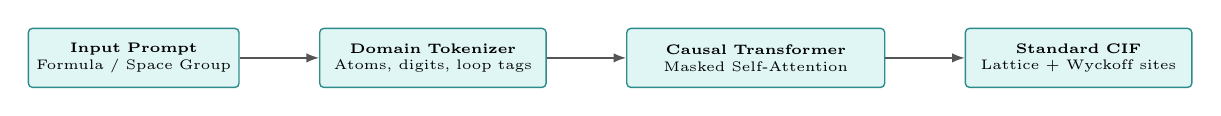
\begin{tikzpicture}[x=1cm,y=1cm]
  \node[battbox, text width=2.5cm, minimum height=0.75cm] (p) at (0,0) {\textbf{Input Prompt} \\ {\tiny Formula / Space Group}};
  \node[battbox, text width=2.7cm, minimum height=0.75cm] (tok) at (3.8,0) {\textbf{Domain Tokenizer} \\ {\tiny Atoms, digits, loop tags}};
  \node[battbox, text width=3.1cm, minimum height=0.75cm] (llm) at (7.9,0) {\textbf{Causal Transformer} \\ {\tiny Masked Self-Attention}};
  \node[battbox, text width=2.7cm, minimum height=0.75cm] (cif) at (12.0,0) {\textbf{Standard CIF} \\ {\tiny Lattice + Wyckoff sites}};

  \draw[flowarrow] (p) -- (tok);
  \draw[flowarrow] (tok) -- (llm);
  \draw[flowarrow] (llm) -- (cif);
\end{tikzpicture}}

\vspace{0.35cm}
\begin{columns}[T]
    \column{0.49\textwidth}
    \footnotesize
    \textbf{Token-by-Token Autoregression:}
    \vspace{0.15cm}
    \begin{itemize}\itemsep0.8em
        \item Predicts the next token based on all preceding context:
        $$P(\mathbf{x}) = \prod_{t=1}^{T} P(x_t \mid x_1, \dots, x_{t-1}; \theta)$$
        \item Emits one character or coordinate at a time until the entire 3D crystal file is complete.
    \end{itemize}

    \column{0.49\textwidth}
    \footnotesize
    \textbf{The Vanilla Baseline Mechanism:}
    \vspace{0.15cm}
    \begin{itemize}\itemsep0.5em
        \item \textbf{Causal Self-Attention:} Computes attention strictly between past text tokens to learn local bond lengths and angles.
        \item \textbf{The Core Limitation:} Over long CIF sequences ($> 500$ tokens for 20+ atoms), attention attenuates and forgets initial constraints.
        \item \textbf{Motivation for Modification:} Needs persistent external guidance throughout the sequence to maintain target battery properties.
    \end{itemize}
\end{columns}
\end{frame}

% ============================================================
% SLIDE 18: COMBINED SLIDE: CROSS-ATTENTION MECHANISM & ARCHITECTURE
% ============================================================
\begin{frame}{Our Modifications to CrystaLLM: Cross-Attention Injection~\cite{antunes2024crystallm}}
\framesubtitle{Steering crystal generation with ontology knowledge at every transformer layer}
\vspace{-0.15cm}

\centering
\resizebox{0.88\linewidth}{!}{%
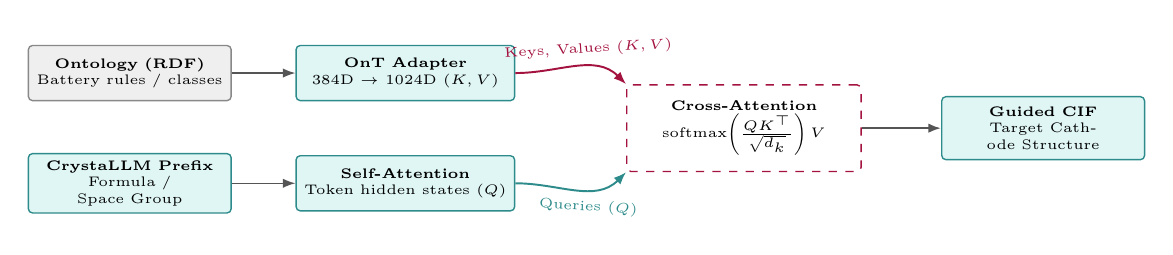
\begin{tikzpicture}[x=1cm,y=1cm]
  % Top Branch: Ontology Knowledge
  \node[emmobox, text width=2.4cm, minimum height=0.7cm] (ont_kg) at (0, 1.0) {\textbf{Ontology (RDF)} \\ {\tiny Battery rules / classes}};
  \node[battbox, text width=2.6cm, minimum height=0.7cm] (ont) at (3.5, 1.0) {\textbf{OnT Adapter} \\ {\tiny 384D $\to$ 1024D ($K, V$)}};

  % Bottom Branch: CrystaLLM Self-Attention
  \node[battbox, text width=2.4cm, minimum height=0.7cm] (cif_in) at (0, -0.4) {\textbf{CrystaLLM Prefix} \\ {\tiny Formula / Space Group}};
  \node[battbox, text width=2.6cm, minimum height=0.7cm] (self) at (3.5, -0.4) {\textbf{Self-Attention} \\ {\tiny Token hidden states ($Q$)}};

  % Center Fusion: Cross-Attention
  \node[gapbox, text width=2.8cm, minimum height=1.1cm] (cross) at (7.8, 0.3) {\textbf{Cross-Attention} \\ {\tiny $\mathrm{softmax}\!\left(\frac{QK^\top}{\sqrt{d_k}}\right)V$}};

  % Output: Final CIF
  \node[battbox, text width=2.4cm, minimum height=0.8cm] (out) at (11.6, 0.3) {\textbf{Guided CIF} \\ {\tiny Target Cathode Structure}};

  % Connections
  \draw[flowarrow] (ont_kg) -- (ont);
  \draw[flowarrow] (cif_in) -- (self);
  \draw[flowarrow, draw=amritaMaroon, line width=0.7pt] (ont.east) to[out=0, in=135] node[above, font=\tiny, text=amritaMaroon, sloped, xshift=5pt]{Keys, Values ($K,V$)} (cross.north west);
  \draw[flowarrow, draw=battCyanLine, line width=0.7pt] (self.east) to[out=0, in=-135] node[below, font=\tiny, text=battCyanLine, sloped, xshift=5pt]{Queries ($Q$)} (cross.south west);
  \draw[flowarrow, line width=0.8pt] (cross) -- (out);
\end{tikzpicture}}

\vspace{0.25cm}
\begin{columns}[T]
    \column{0.50\textwidth}
    \footnotesize
    Attention operates as a \textbf{soft dictionary lookup}:
    \vspace{0.15cm}
    \begin{itemize}\itemsep0.35em
        \item \textbf{Query $Q$:} What the current crystal token is looking for (from CrystaLLM hidden states).
        \item \textbf{Key $K$:} What each ontology concept advertises about itself (from OnT embeddings).
        \item \textbf{Value $V$:} What structural constraints the ontology hands over to steer generation.
    \end{itemize}

    \column{0.48\textwidth}
    \footnotesize
    \textbf{Mathematical Formulation:}
    $$\mathrm{Attn}(Q,K,V) = \mathrm{softmax}\!\left(\frac{QK^{\top}}{\sqrt{d_k}}\right)V$$
    \vspace{-0.1cm}
    \begin{itemize}\itemsep0.35em
        \item \textbf{Continuous Steering:} Injected into every transformer layer so CrystaLLM references cathode rules at each token step.
    \end{itemize}
\end{columns}
\end{frame}

% ============================================================
% SLIDE: SYSTEM ARCHITECTURE
% ============================================================
\begin{frame}{System Architecture}
\framesubtitle{End-to-end component view: knowledge $\to$ conditioning $\to$ generation $\to$ validation}
\centering
\vspace{0.3cm}
\resizebox{0.95\linewidth}{!}{%
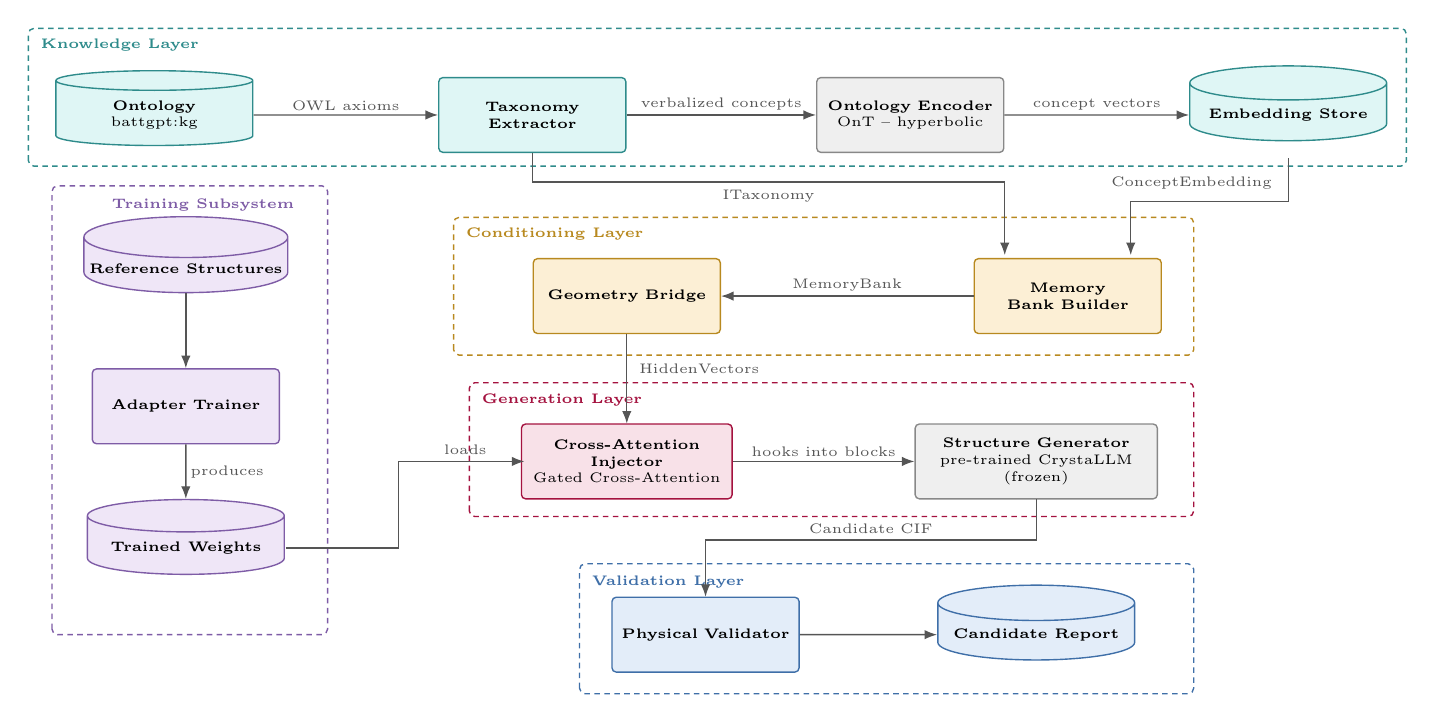
\begin{tikzpicture}[x=1cm,y=1cm]

  % ---------- layer containers ----------
  \draw[layerbox=battCyanLine]  (-0.6,5.95) rectangle (16.9,7.7);
  \draw[layerbox=condLine]      (4.8,3.55)  rectangle (14.2,5.3);
  \draw[layerbox=trainLine]     (-0.3,0.0)  rectangle (3.2,5.7);
  \draw[layerbox=genLine]       (5.0,1.5)   rectangle (14.2,3.2);
  \draw[layerbox=valLine]       (6.4,-0.75) rectangle (14.2,0.9);

  \node[layerlabel=battCyanLine] at (-0.5,7.62) {Knowledge Layer};
  \node[layerlabel=condLine]     at (4.9,5.22)  {Conditioning Layer};
  \node[layerlabel=trainLine]    at (0.4,5.60) {Training Subsystem};
  \node[layerlabel=genLine]      at (5.1,3.12)  {Generation Layer};
  \node[layerlabel=valLine]      at (6.5,0.80)  {Validation Layer};

  % ---------- knowledge layer ----------
  \node[archstore={battCyanLine}{battCyan}] (ont)   at (1.0,6.6)  {\textbf{Ontology} \\ {\tiny battgpt:kg}};
  \node[archnode={battCyanLine}{battCyan}]  (tax)   at (5.8,6.6)  {\textbf{Taxonomy Extractor}};
  \node[archnode={emmoGreyLine}{emmoGrey}]  (enc)   at (10.6,6.6) {\textbf{Ontology Encoder} \\ {\tiny OnT -- hyperbolic}};
  \node[archstore={battCyanLine}{battCyan}] (store) at (15.4,6.6) {\textbf{Embedding Store}};

  % ---------- conditioning layer ----------
  \node[archnode={condLine}{condFill}] (geom) at (7.0,4.3)  {\textbf{Geometry Bridge}};
  \node[archnode={condLine}{condFill}] (mbb)  at (12.6,4.3) {\textbf{Memory Bank Builder}};

  % ---------- training subsystem ----------
  \node[archstore={trainLine}{trainFill}] (refs)  at (1.4,4.65) {\textbf{Reference Structures}};
  \node[archnode={trainLine}{trainFill}]  (train) at (1.4,2.9) {\textbf{Adapter Trainer}};
  \node[archstore={trainLine}{trainFill}] (wts)   at (1.4,1.1) {\textbf{Trained Weights}};

  % ---------- generation layer ----------
  \node[archnode={genLine}{genFill}, text width=2.5cm] (inj) at (7.0,2.2) {\textbf{Cross-Attention Injector} \\ {\tiny Gated Cross-Attention}};
  \node[archnode={emmoGreyLine}{emmoGrey}, text width=2.9cm] (gen) at (12.2,2.2) {\textbf{Structure Generator} \\ {\tiny pre-trained CrystaLLM} \\ {\tiny (frozen)}};

  % ---------- validation layer ----------
  \node[archnode={valLine}{valFill}]  (val) at (8.0,0.0)  {\textbf{Physical Validator}};
  \node[archstore={valLine}{valFill}] (rep) at (12.2,0.0) {\textbf{Candidate Report}};

  % ---------- knowledge flow ----------
  \draw[flowarrow] (ont) -- node[archlabel,above]{OWL axioms} (tax);
  \draw[flowarrow] (tax) -- node[archlabel,above]{verbalized concepts} (enc);
  \draw[flowarrow] (enc) -- node[archlabel,above]{concept vectors} (store);

  % ---------- knowledge -> conditioning ----------
  \draw[flowarrow] (5.8,6.12) -- (5.8,5.75) -- (11.8,5.75) -- (11.8,4.82);
  \node[archlabel,anchor=north] at (8.8,5.71) {ITaxonomy};

  \draw[flowarrow] (15.4,6.05) -- (15.4,5.50) -- (13.4,5.50) -- (13.4,4.82);
  \node[archlabel,anchor=east] at (15.25,5.74) {ConceptEmbedding};

  \draw[flowarrow] (mbb) -- node[archlabel,above]{MemoryBank} (geom);

  % ---------- conditioning -> generation ----------
  \draw[flowarrow] (7.0,3.82) -- (7.0,2.68);
  \node[archlabel,anchor=west] at (7.1,3.38) {HiddenVectors};

  % ---------- training subsystem ----------
  \draw[flowarrow] (refs) -- (train);
  \draw[flowarrow] (train) -- node[archlabel,right]{produces} (wts);
  \draw[flowarrow] (2.67,1.1) -- (4.1,1.1) -- (4.1,2.2) -- (5.70,2.2);
  \node[archlabel,anchor=south] at (4.95,2.23) {loads};

  % ---------- generation ----------
  \draw[flowarrow] (inj) -- node[archlabel,above]{hooks into blocks} (gen);

  % ---------- generation -> validation ----------
  \draw[flowarrow] (12.2,1.72) -- (12.2,1.20) -- (8.0,1.20) -- (8.0,0.48);
  \node[archlabel,anchor=south] at (10.1,1.23) {Candidate CIF};

  \draw[flowarrow] (val) -- (rep);

\end{tikzpicture}}

\end{frame}

% ============================================================
% SECTION: CRYSTAL GENERATION
% ============================================================
\section{Crystal Generation}

\begin{frame}{From Formula Generation to Crystal Discovery}
    \framesubtitle{Oxidation-State Enumeration as the Bridge to Structure Generation}

    \begin{center}
        \textbf{\large Formula obtained from Knowledge-Conditioned CrystaLLM}

        \vspace{0.10cm}

        \[
        \boxed{\text{Chemical Formula}}
        \quad\longrightarrow\quad
        \boxed{\text{Oxidation-State Enumeration}}
        \quad\longrightarrow\quad
        \boxed{\text{MatterGen}} \cite{mattergen2025}
        \]
    \end{center}

    \vspace{0.02cm}

    \begin{columns}[T]

        \column{0.47\textwidth}

        \textbf{\large Input to the Materials Pipeline}

        \vspace{0.03cm}

        {\small
        \begin{itemize}
            \setlength{\itemsep}{3pt}
            \setlength{\parskip}{0pt}

            \item
            \textbf{Chemical formula} obtained from CrystaLLM.

            \item The formula defines the target
            \textbf{elemental composition}.

            \item The composition is used to enumerate
            \textbf{chemically feasible oxidation-state configurations}.
        \end{itemize}
        }

        \column{0.47\textwidth}

        \textbf{\large Why Oxidation-State Enumeration?}

        \vspace{0.03cm}

        {\small
        \begin{itemize}
            \setlength{\itemsep}{3pt}
            \setlength{\parskip}{0pt}

            \item A composition can admit
            \textbf{multiple oxidation-state configurations}.

            \item Each valid configuration represents a
            \textbf{distinct electronic constraint}.

            \item Each configuration becomes a
            \textbf{conditioning input} for crystal generation.
        \end{itemize}
        }

    \end{columns}

    \vfill

\end{frame}


% ============================================================
% SECTION: FINE-TUNING (declared once)
% ============================================================
\section{Fine-Tuning}

\begin{frame}{MatterGen Adapter Fine-Tuning}
    \framesubtitle{Leveraging Parameter-Efficient Conditioning of the Pretrained Generator}

    \begin{columns}[T]

        \column{0.37\textwidth}

        \textbf{Why Fine-Tune MatterGen?}

        \vspace{0.02cm}

        {\footnotesize
        \begin{itemize}
            \setlength{\itemsep}{0pt}

            \item MatterGen is a pretrained diffusion model for
            inorganic crystal structure generation.

            \item The pretrained model does not explicitly condition
            generation on \textbf{oxidation states}.

            \item MatterGen provides an existing
            \textbf{adapter-based fine-tuning architecture}.

            \item We leverage this architecture to introduce
            \textbf{oxidation-state conditioning}.
        \end{itemize}
        }

        \vspace{0.02cm}

        \begin{block}{\scriptsize Key Idea}
            \centering
            \scriptsize
            \textbf{Adapt the pretrained generator}\\
            without retraining the complete model.
        \end{block}

        \column{0.59\textwidth}

        \textbf{\large General Adapter Mechanism}

        \vspace{0.08cm}

        \begin{center}
            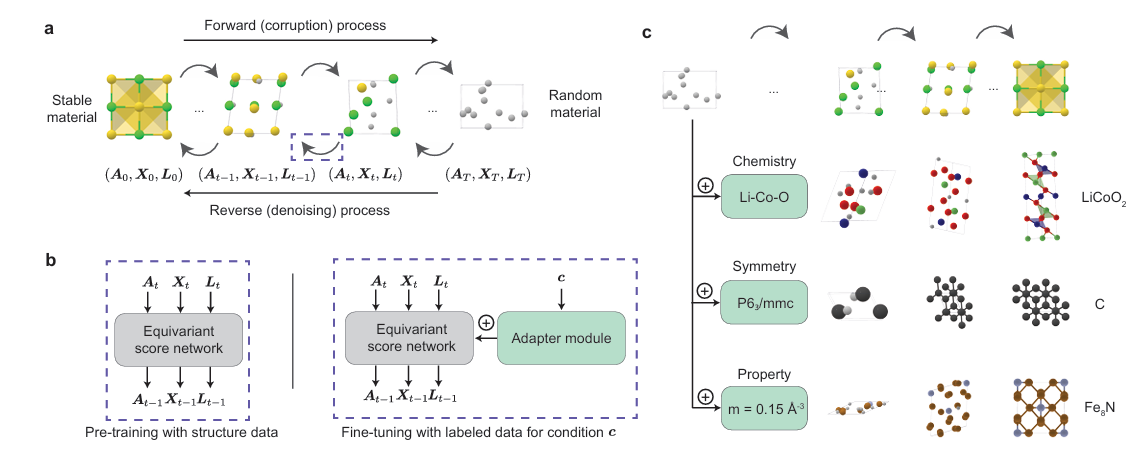
\includegraphics[
                width=\textwidth,
                height=5.0cm,
                keepaspectratio
            ]{image.png}
        \end{center}

        \vspace{0.05cm}

        \centering
        \scriptsize
        \textit{General adapter-based conditioning mechanism used by
        the pretrained architecture.}
        \cite{mattergen2025}
    \end{columns}


\end{frame}

\begin{frame}{Oxidation-State Conditioning Architecture}
    \framesubtitle{Adapting MatterGen to Generate Structures Under Oxidation-State Conditions}

    \begin{columns}[T]

        \column{0.40\textwidth}

        \textbf{\large Oxidation-State Conditioning}

        \vspace{0.02cm}

        {\footnotesize
        \begin{enumerate}
            \setlength{\itemsep}{1pt}
            \setlength{\parskip}{0pt}

            \item \textbf{Oxidation-State Encoding}\\[-2pt]
            Each configuration is represented as a categorical vector.

            \item \textbf{Embedding}\\[-2pt]
            The encoded configuration is mapped to a dense
            oxidation-state representation.

            \item \textbf{Adapter MLP}\\[-2pt]
            Learns how oxidation-state information influences the
            pretrained representation.

            \item \textbf{Zero-Initialized Mix-in}\\[-2pt]
            Injects the adapter output into the GemNet
            message-passing layers.
        \end{enumerate}
        }

        \vspace{0.02cm}

        \begin{block}{\centering \footnotesize Parameter-Efficient Training}
            \centering
            \scriptsize
            \textbf{Backbone: Frozen}
            \quad|\quad
            \textbf{Adapters: Trainable}
        \end{block}

        \column{0.56\textwidth}

        \textbf{\large Adapter Integration}

        \vspace{0.02cm}

        \begin{center}
            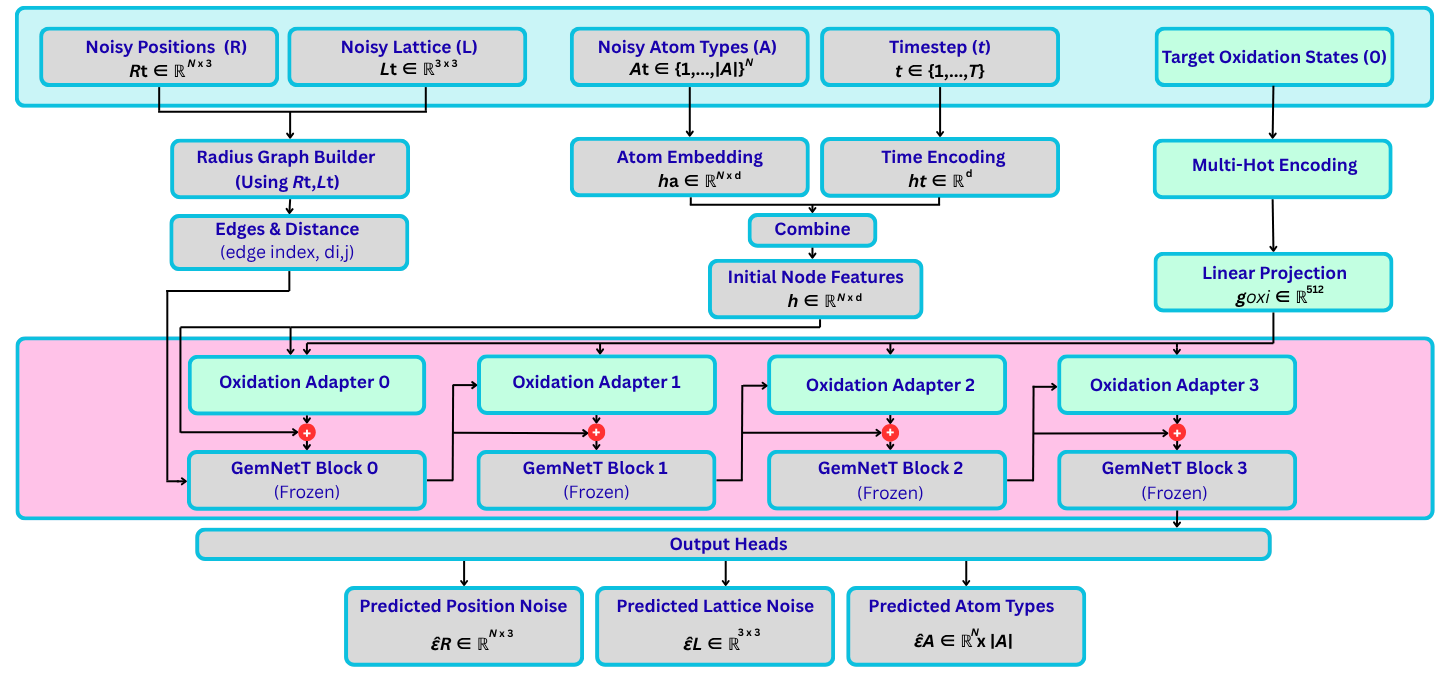
\includegraphics[
                width=\textwidth,
                height=4.10cm,
                keepaspectratio
            ]{adapter.png}
            \cite{mattergen2025}
        \end{center}
    \end{columns}


\end{frame}

\begin{frame}{Fine-Tuning Dataset \& Evaluation}
    \framesubtitle{Oxidation-State Labelling and Generation Consistency}

    \begin{columns}[T]

        \column{0.47\textwidth}

        \textbf{\large Dataset Construction}

        \vspace{0.03cm}

        {\footnotesize
        \begin{enumerate}
            \setlength{\itemsep}{1pt}

            \item \textbf{MP20}\\[-2pt]
            Lithium-based transition-metal oxide
            structures were extracted.

            \item \textbf{Oxidation-State Labelling}\\[-2pt]
            Oxidation states were assigned using
            \textbf{bond-valence analysis}\cite{pymatgen2013}.

            \item \textbf{Quality Filtering}\\[-2pt]
            Structures with \textbf{fractional or ambiguous}
            oxidation states were discarded.

            \item \textbf{Final Dataset}\\[-2pt]
            Remaining structures were used for
            oxidation-state-conditioned fine-tuning.
        \end{enumerate}
        }

        \vspace{0.04cm}

        \begin{block}{\footnotesize Training Dataset}
            \centering
            \footnotesize
            MP20 $\rightarrow$ Li--O structures
            $\rightarrow$ oxidation-state labelling
            $\rightarrow$ quality filtering
        \end{block}

        \column{0.49\textwidth}

\textbf{\large Generation \& Evaluation}

\vspace{0.03cm}

{\footnotesize
\begin{itemize}
    \setlength{\itemsep}{2pt}

    \item \textbf{1000} structures generated for \textbf{Li--TM--O}.

    \item Composition filtering: \textbf{120 formulas}.

    \item Oxidation-state enumeration\cite{pymatgen2013}: \textbf{146 pairs}.

    \item \textbf{20 structures/pair} $\rightarrow$ \textbf{2920 structures}.

    \item \textbf{1000} oxidation-state mismatches.

    \item \textbf{1920} structures matched target oxidation states.

\end{itemize}
}

\vspace{0.04cm}

\begin{block}{\footnotesize Oxidation-State Consistency}
    \centering
    \normalsize
    \textbf{1920 / 2920 = 65.75\%}\\[1pt]
    \footnotesize
    structures matched the target configuration
\end{block}

\end{columns}



\end{frame}

% ============================================================
% SECTION: RESULTS
% ============================================================
\section{Results}

\begin{frame}{Hierarchical Screening \& Candidate Selection}
    \framesubtitle{Progressive Filtering from Generated Structures to Experimental Validation}

    \centering

    \begin{tabular}{c@{\quad$\rightarrow$\quad}c@{\quad$\rightarrow$\quad}c@{\quad$\rightarrow$\quad}c@{\quad$\rightarrow$\quad}c}

        \begin{minipage}{1.40cm}
            \centering
            \textbf{Generated}\\
            \textbf{2920}\\
            \scriptsize
            OS-conditioned
        \end{minipage}

        &

        \begin{minipage}{1.40cm}
            \centering
            \textbf{OS Match}\\
            \textbf{1920}\\
            \scriptsize
            Target OS\\
            consistent
        \end{minipage}

        &

        \begin{minipage}{1.40cm}
            \centering
            \textbf{MLFF}\\
            \textbf{580}\\
            \scriptsize
            $E_{\mathrm{hull}}\leq0.10$\\
            eV/atom
        \end{minipage}

        &

        \begin{minipage}{1.40cm}
            \centering
            \textbf{S.U.N.}\\
            \textbf{99}\\
            \scriptsize
            Stable +\\
            Unique + Novel
        \end{minipage}

        &

        \begin{minipage}{1.40cm}
            \centering
            \textbf{DFT}\\
            \textbf{29}\\
            \scriptsize
            $E_{\mathrm{hull}}\leq0.03$\\
            eV/atom
        \end{minipage}

    \end{tabular}

    \vspace{0.32cm}

    \begin{columns}[T]

        \column{0.32\textwidth}

        \textbf{1. MLFF Screening}

        \vspace{0.01cm}

        {\footnotesize
        \begin{itemize}
            \setlength{\itemsep}{1pt}

            \item Relaxation using
            \textbf{MatterSim MLFF}. \cite{mattersim2024}

            \item Stability evaluated using
            energy above convex hull.

            \item \textbf{580} structures:
            $E_{\mathrm{hull}}\leq0.10\,\mathrm{eV/atom}$.
        \end{itemize}
        }

        \column{0.34\textwidth}

        \textbf{2. S.U.N. Screening} \cite{battery_mattergen2025}

        \vspace{0.01cm}

        {\footnotesize
        \begin{itemize}
            \setlength{\itemsep}{1pt}

            \item \textbf{Stable:} energetically
            favourable structures.

            \item \textbf{Unique:} remove duplicate
            polymorphs.

            \item \textbf{Novel:} remove previously
            reported structures.

            \item \textbf{580 $\rightarrow$ 99}
        \end{itemize}
        }

        \column{0.32\textwidth}

        \textbf{3. DFT Validation}\cite{battery_mattergen2025}

        \vspace{0.01cm}

        {\footnotesize
        \begin{itemize}
            \setlength{\itemsep}{1pt}

            \item Full DFT relaxation and
            stability evaluation.

            \item \textbf{29} structures:
            $E_{\mathrm{hull}}\leq0.03\,\mathrm{eV/atom}$.

            \item Electrochemical analysis
            performed on the 29 candidates.
        \end{itemize}
        }

    \end{columns}

    \vspace{0.02cm}

    \begin{beamercolorbox}[
        rounded=true,
        sep=3pt
    ]{block body}

        \centering
        \small
        \textbf{Selected: Li$_3$Mn$_2$NiO$_6$}
        \quad|\quad
        \textbf{281.74 mAh/g}
        \quad|\quad
        \textbf{3.451 V}
        \quad|\quad
        \textbf{$E_{\mathrm{hull}}=0.0227$ eV/atom}

    \end{beamercolorbox}

    \vspace{0.03cm}

    \centering
    \scriptsize
    \textbf{Experimental Validation:}
    Li$_3$Mn$_2$NiO$_6$ was synthesized and characterized by XRD.

\end{frame}

\begin{frame}{Next Milestones}
\framesubtitle{Closing the ontology loop, and proving the conditioning works}
\scriptsize
\begin{columns}[T]
    \column{0.46\textwidth}
    {\footnotesize \textbf{\textcolor{battCyanLine}{Ontology track}}}
    \vspace{0.2cm}
    \begin{enumerate}\itemsep0.45em
        \item \textbf{Broaden instance coverage} beyond the current cathode slice, populating every battery role and structural family, not just cathodes.
        \item \textbf{Validate against every competency question} by running each one as a real query against the populated graph, closing the engineering loop end-to-end.
        \item \textbf{Keep enriching structural semantics} so structure-family membership carries real geometric and crystallographic meaning, not just a taxonomic label.
        \item \textbf{Score the ontology against OQuaRE} to benchmark its structural and design quality against established ontology-evaluation metrics.
    \end{enumerate}

    \column{0.5\textwidth}
    {\footnotesize \textbf{\textcolor{amritaMaroon}{Conditioning pipeline}}}
    \vspace{0.2cm}
    \begin{enumerate}\itemsep0.45em
        \item \textbf{OnT -- extend to the populated KG.} The encoder currently embeds the \textbf{TBox}; extend it toward \textbf{ABox instance embeddings} by verbalizing material entities and reusing its hierarchy and role mechanisms.
        \item \textbf{Generation -- widen the target set.} Run conditioned CrystaLLM for at least one generation target per \texttt{StructureFamily} leaf.
        \item \textbf{Output -- demonstrate ontology-driven generation.} Show generated CIFs landing in the requested family, turning ``the ontology is wired in'' into ``the ontology changes what comes out.''
        \item \textbf{Seed the MatterGen track} with formulas extracted from conditioned output, completing the planned merger.
    \end{enumerate}
\end{columns}
\end{frame}

% ============================================================
% SECTION: TECHNICAL ENRICHMENT
% ============================================================
\section{Technical Enrichment}

\begin{frame}{Technical Enrichment Activity Choices}
    \framesubtitle{Professional Online Certification Details (Individual Mandatory: 10--20 Hours)}
    \begin{itemize}
        \item \textbf{Individual MOOC / Online Certification Selection:}
    \end{itemize}
    \vspace{-0.1cm}
    \begin{table}
        \centering
        \footnotesize
        \renewcommand{\arraystretch}{1.15}
        \begin{tabular}{|c|p{2.8cm}|p{5.0cm}|p{2.3cm}|c|}
            \hline
            \textbf{S.No} & \textbf{Student Name} & \textbf{Chosen MOOC / Course Title} & \textbf{Platform} & \textbf{Hours} \\
            \hline
            1 & Akshay KS & Knowledge Graphs -- Foundations and Applications & openHPI & 15 Hrs \\
            \hline
            2 & R.D.Tarun & Knowledge Graphs -- Foundations and Applications & openHPI & 15 Hrs \\
            \hline
            3 & S Ajeth & Knowledge Graphs -- Foundations and Applications & openHPI & 15 Hrs \\
            \hline
            4 & Sarvesha NK & Knowledge Graphs -- Foundations and Applications & openHPI & 15 Hrs \\
            \hline
            5 & Shantharam P & Knowledge Graphs -- Foundations and Applications & openHPI & 15 Hrs \\
            \hline
        \end{tabular}
    \end{table}
    \vspace{0.1cm}
    \begin{itemize}
        \item {\scriptsize \textbf{Course:} \url{https://open.hpi.de/courses/knowledgegraphs2023} -- all five team members have registered for this course together, directly relevant to the ontology and knowledge-graph track of this project.}
    \end{itemize}
\end{frame}

% --- REFERENCES ---
\section{References}
\begin{frame}[allowframebreaks]{References}
    \nocite{xiong2022boxel,jackermeier2024dual,wang2022simkgc,wang2021kepler,hu2020hgt,sun2019rotate,tang2024rule,battery_mattergen2025,mattersim2024,mattergen2025,antunes2024crystallm,emmo2024,clark2022battinfo,jain2013materialsproject,kazakov2014elk,yang2025ont}
    \bibliographystyle{IEEEtran}
    \bibliography{ref}
\end{frame}

% --- THANK YOU ---
\begin{frame}
    \centering
    {\Huge \textbf{\textcolor{amritaMaroon}{Thank You}}}
\end{frame}

\end{document}
